\subsection{Porucha harmonického oscilátoru}
Částice hmotnosti $M$ se pohybuje v potenciálu jednorozměrného lineárního harmonického oscilátoru
\begin{equation}
    \operator{V}_{0}=\frac{1}{2}M\Omega^{2}\operator{x}^{2}
\end{equation}
s malou poruchou
\begin{equation}
    \operator{V}_{\mathrm{I}}=\lambda\cos\left(\kappa\operator{x}+\varphi\right)\,.
\end{equation}
\begin{enumerate}
\item
    Spočítejte 1. řád opravy energie základního stavu.
    
\item
    Vyjádřete střední hodnotu operátoru souřadnice $\operator{x}$ a střední hodnotu kvadrátu operátoru souřadnice $\operator{x}^{2}$ v tomto stavu.
\end{enumerate}

\begin{solution}
	\begin{enumerate}
	\item
		Oprava k energii je podle~\eqref{eq:Perturbation1}
		\begin{equation}
			E_{0}^{(1)}
				=\matrixelement{0}{\cos\left(\kappa\operator{x}+\varphi\right)}{0}
				=\real\matrixelement{0}{\e^{\im\kappa\operator{x}}\e^{\im\varphi}}{0}
				=\real\left[\e^{\im\varphi}\matrixelement{0}{\e^{\im\kappa\operator{x}}}{0}\right]
		\end{equation}		
		(neporušenou bázi harmonického oscilátoru značíme v souladu s dříve užívanou konvencí $\ket{\phi_{n}}\equiv\ket{n}$, $n=0,1,2,\dotsc$).
		Operátor souřadnice vyjádříme pomocí posunovacích operátorů $\operator{a},\conjugate{\operator{a}}$ [vztah~\eqref{eq:PXToShiftOperator}]
		\begin{equation}
			\operator{x}=\sqrt{\frac{\hbar}{2M\Omega}}\left(\conjugate{\operator{a}}+\operator{a}\right)
		\end{equation}
		a použijeme \trick{Baker-Campbell-Hausdorffovu formuli}~\eqref{eq:BCH1}
        \begin{subequations}
            \begin{align}
                \e^{\operator{A}+\operator{B}}
                    &=\e^{\operator{A}}\e^{\operator{B}}\e^{-\frac{1}{2}\commutator{\operator{A}}{\operator{B}}},\\
                \operator{A}
                    &\equiv\im\kappa\sqrt{\frac{\hbar}{2M\Omega}}\conjugate{\operator{a}},\\
                \operator{B}
                    &\equiv\im\kappa\sqrt{\frac{\hbar}{2M\Omega}}\operator{a},\\
                \commutator{\operator{A}}{\operator{B}}
                    &=-\kappa^{2}\frac{\hbar}{2M\Omega}\underbrace{\commutator{\conjugate{\operator{a}}}{\operator{a}}}_{-1},\\
            \end{align}            
        \end{subequations}
		takže
		\begin{equation}
			\label{eq:HOPerturbedBCH}
			\e^{\im\kappa\operator{x}}
				=\e^{\im\kappa\sqrt{\frac{\hbar}{2M\Omega}}\conjugate{\operator{a}}}\e^{\im\kappa\sqrt{\frac{\hbar}{2M\Omega}}\operator{a}}\e^{-\kappa^{2}\frac{\hbar}{4M\Omega}}
		\end{equation}
		a 
		\begin{align}
			E_{0}^{(1)}
				&=\Re\left[\e^{\im\varphi}\e^{-\kappa^{2}\frac{\hbar}{4M\Omega}}\matrixelement{0}{\e^{\im\kappa\sqrt{\frac{\hbar}{2M\Omega}}\conjugate{\operator{a}}}\e^{\im\kappa\sqrt{\frac{\hbar}{2M\Omega}}\operator{a}}}{0}\right]\nonumber\\
				&=\Re\left[\e^{\im\varphi}\e^{-\kappa^{2}\frac{\hbar}{4M\Omega}}\matrixelement{0}{\left(\operator{1}+\im\kappa\sqrt{\frac{\hbar}{2M\Omega}}\conjugate{\operator{a}}+\dotsb\right)\left(\operator{1}+\im\kappa\sqrt{\frac{\hbar}{2M\Omega}}\operator{a}+\dotsb\right)}{0}\right]\nonumber\\
				&=\e^{-\kappa^{2}\frac{\hbar}{4M\Omega}}\cos{\varphi}.
		\end{align}
		Pokud je $\phi=k\pi$, $k\in\mathbb{Z}$ je první oprava k energii základního stavu nejvyšší (porucha je sudá funkce),
		pokud naopak $\phi=k\pi+\pi/2$, je oprava nulová (porucha je lichá funkce).
	
		\begin{figure}[!htbp]
			\centering
			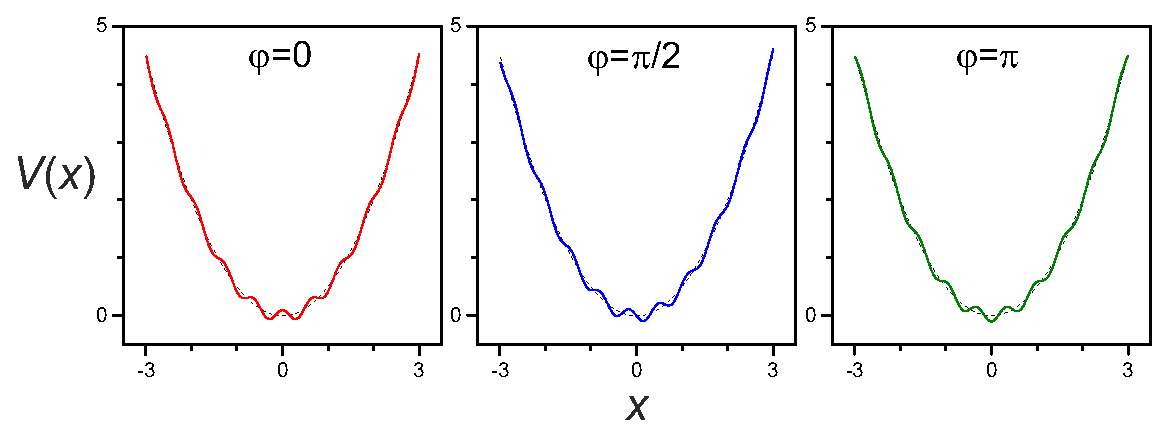
\epsfig{file=figures/porucha.eps,width=\linewidth,keepaspectratio}
			\scaption{
				Potenciál $V(x)=V_{0}(x)+V_{\mathrm{I}}(x)$ pro tři hodnoty fáze $\varphi$ (silnou barevnou čarou)
				a neporušený potenciál $V_{0}(x)$ (čárkovanou černou čarou).
				Hodnoty parametrů jsou $M=\Omega=1$, $\kappa=10$, $\lambda=0,\!1$.
				Při volbě $\hbar=0.1$ je energie neporušeného základního stavu $E_{0}^{(0)}=0,\!05$ a poruchy v jednotlivých případech
				$E_{0}^{(1)}=\left\{0,\!0082;0;-0,\!0082\right\}$.
				Střední hodnota souřadnice se posune o $0,\!082$ v případě $\varphi=\pi/2$, ve zbylých dvou případech zůstane nulová.
			}
			\label{fig:HOporucha}
		\end{figure}
	
	\item
		Oprava k vlastnímu vektoru základního stavu je podle~\eqref{eq:Perturbation1}
		\begin{equation}
			\ket{\chi_{0}^{(1)}}
				=\sum_{n=1}^{\infty}\frac{\matrixelement{n}{\cos\left(\kappa\operator{x}+\varphi\right)}{0}}{E_{0}^{(0)}-E_{n}^{(0)}}\ket{n}
				=-\frac{1}{\hbar\Omega}\sum_{n=1}^{\infty}\frac{1}{n}\Re\left[\e^{\im\varphi}\matrixelement{n}{\e^{\im\kappa\operator{x}}}{0}\right]\ket{n}\,.
		\end{equation}
		Využijeme vztahu~\eqref{eq:HOPerturbedBCH}, a maticový element v sumě vyjádříme jako
		\begin{align}
				\matrixelement{n}{\e^{\im\kappa\operator{x}}}{0}
					&=\e^{-\kappa^{2}\frac{\hbar}{4M\Omega}}\matrixelement{n}{\e^{\im\kappa\sqrt{\frac{\hbar}{2M\Omega}}\conjugate{\operator{a}}}\e^{\im\kappa\sqrt{\frac{\hbar}{2M\Omega}}\operator{a}}}{0}\nonumber\\
					&=\e^{-\kappa^{2}\frac{\hbar}{4M\Omega}}\matrixelement{n}{\e^{\im\kappa\sqrt{\frac{\hbar}{2M\Omega}}\conjugate{\operator{a}}}}{0}\nonumber\\
					&=\e^{-\kappa^{2}\frac{\hbar}{4M\Omega}}\matrixelement{n}{\sum_{k=0}^{\infty}\frac{1}{k!}\left(\im\kappa\sqrt{\frac{\hbar}{2M\Omega}}\right)^{k}\operator{a}^{\dagger k}}{0}\nonumber\\
					&=\frac{\e^{-\kappa^{2}\frac{\hbar}{4M\Omega}}}{\sqrt{n!}}\left(\im\kappa\sqrt{\frac{\hbar}{2M\Omega}}\right)^{n}\,,
			\end{align}
			takže
			\begin{align}
				\ket{\chi_{0}^{(1)}}
					&=-\frac{1}{\hbar\Omega}\sum_{n=1}^{\infty}\frac{1}{n}\frac{\e^{-\kappa^{2}\frac{\hbar}{4M\Omega}}}{\sqrt{n!}}\Re\left[\e^{\im\varphi}\left(\im\kappa\sqrt{\frac{\hbar}{2M\Omega}}\right)^{n}\right]\ket{n}\nonumber\\
					&=-\frac{1}{\hbar\Omega}\e^{-\kappa^{2}\frac{\hbar}{4M\Omega}}\sum_{n=1}^{\infty}\frac{1}{n\sqrt{n!}}\Re\left[\left(\cos{\varphi}+\im\sin{\varphi}\right)\left(\im\kappa\sqrt{\frac{\hbar}{2M\Omega}}\right)^{n}\right]\ket{n}\nonumber\\
					&=-\frac{1}{\hbar\Omega}\e^{-\kappa^{2}\frac{\hbar}{4M\Omega}}\left[
						\cos{\varphi}\sum_{n=1}^{\infty}\frac{\minus{n}}{2n\sqrt{(2n)!}}\kappa^{2n}\left(\frac{\hbar}{2M\Omega}\right)^{n}\ket{2n}\right.\nonumber\\
					&\qquad\left.-\sin{\varphi}\sqrt{\frac{\hbar}{2M\Omega}}\sum_{n=0}^{\infty}\frac{\minus{n}}{(2n+1)\sqrt{(2n+1)!}}\kappa^{2n+1}\left(\frac{\hbar}{2M\Omega}\right)^{n}\ket{2n+1}\right].
			\end{align}
			Střední hodnota operátoru souřadnice je tedy (do prvního řádu v $\lambda$)
			\begin{align}
				\matrixelement{\chi_{0}}{\operator{x}}{\chi_{0}}
					&=\sqrt{\frac{\hbar}{2M\Omega}}\left[\bra{0}+\lambda\bra{\chi_{0}^{(1)}}\right]\conjugate{\operator{a}}+\operator{a}\left[\ket{0}+\lambda\ket{\chi_{0}^{(1)}}\right]\nonumber\\
					&\approx\lambda\sqrt{\frac{\hbar}{2M\Omega}}\left[\matrixelement{0}{\operator{a}}{\chi_{0}^{(1)}}+\matrixelement{\chi_{0}^{(1)}}{\conjugate{\operator{a}}}{0}\right]\nonumber\\
					&=2\lambda\sqrt{\frac{\hbar}{2M\Omega}}\matrixelement{\chi_{0}^{(1)}}{\conjugate{\operator{a}}}{0}\nonumber\\
					&=2\lambda\sqrt{\frac{\hbar}{2M\Omega}}\frac{1}{\hbar\Omega}\e^{-\kappa^{2}\frac{\hbar}{4M\Omega}}\sin{\varphi}\sqrt{\frac{\hbar}{2M\Omega}}\,\kappa\nonumber\\
					&=\frac{\lambda\kappa}{M\Omega^{2}}\e^{-\kappa^{2}\frac{\hbar}{4M\Omega}}\sin{\varphi}
			\end{align}
			a střední hodnota kvadrátu operátoru souřadnice (opět do prvního řádu v $\lambda$)
			\begin{align}
				\matrixelement{\chi_{0}}{\operator{x}^{2}}{\chi_{0}}
					&\approx\frac{\hbar}{2M\Omega}\left[\matrixelement{0}{\operator{a}\conjugate{\operator{a}}}{0}+2\lambda\matrixelement{\chi_{0}^{(1)}}{\operator{a}^{\dagger 2}}{0}\right]\nonumber\\
					&=\frac{\hbar}{2M\Omega}\left[1+\frac{\lambda\kappa^{2}}{2M\Omega^{2}}\e^{-\kappa^{2}\frac{\hbar}{4M\Omega}}\cos{\varphi}\right]\,.
			\end{align}			

			Výsledky jsou zobrazeny na obrázku~\ref{fig:HOporucha}.
	\end{enumerate}
\end{solution}
